%INSTALL Pygments sudo apt-get install python-pygments


\documentclass[letterpaper,twocolumn,10pt]{article}
\usepackage{usenix,epsfig,endnotes, upgreek, beamerarticle}
	\setbeamercovered{transparent}
\usepackage{listings}
\usepackage{pxfonts}
\usepackage{amsmath}
\usepackage{amssymb}
\usepackage{parskip}
\usepackage{color}
\usepackage{graphicx}
\usepackage[noend,linesnumbered]{algorithm2e}
\begin{document}

%don't want date printed
\date{}

%make title bold and 14 pt font (Latex default is non-bold, 16 pt)
\title{\Large \bf CSE 231 Project 1}

\author{
{\rm Michael Barrow}\\
mbarrow@eng.ucsd.edu\\
University of California, San Diego
\and
{\rm Jules Testard}\\
Second Institution
\and
{Costas Zafarias}\\
aweff
}

\maketitle

% Use the following at camera-ready time to suppress page numbers.
% Comment it out when you first submit the paper for review.
\thispagestyle{empty}


\subsection*{Abstract}
This report describes the implementation and experimental results of custom LLVM passes applied to supplied benchmark programs. The high level concept of each pass is discussed, followed by key implementation details. Finally we offer conjecture on experimental application of these passes. %This is the structure of the benchmark code is evaluated with respect to pass output 

\section{Introduction}

LLVM is a collection of modular compiler tools. The projects original goal was a flexible compilation strategy for arbitrary programming languages able to perform both static and dynamic compilation.\\
This language flexibility is mainly achieved with a common intermediate program representation during the compilation known as LLVM byte code. Source language and target machine independent optimisations can be made to the LLVM byte code, which is the 231 course project subject of interest.\\
%The price of this flexibility is complexity. End to end, using LLVM requires arranging a subset of its modules into a tool-chain sourcing a specific language and targeting a specific machine. The machine may be virtual 
Our prescribed source language is C++ and our target architecture is x86. The project goal is to profile a set of LLVM compiled C++ benchmarks programs using the \textbf{pass} feature of the \textbf{opt} LLVM module.
Three pass functionalities are required:
\begin{itemize}
\item{Collecting static instruction counts}
\item{Collecting dynamic instruction counts}
\item{Profiling branch bias }
\end{itemize}
The required depth of understanding and proficiency in LLVM module code increases incrementally with each of these three functionalities. Therefore the report is split into three mini-reports to focus on the self contained lessons learned from implementing them. Mini-reports have the following sub sections:\\
\begin{itemize}
\item{\textbf{Instrument description: }A high level description of an \textit{algorithm} used to implement functionality}
\item{\textbf{Instrument implementation summary: }Details on key LLVM concepts and api's used to implement the functionality \textit{algorithm} as an \textit{opt pass}}
\item{\textbf{Benchmark analysis: }Conjecture based running the \textit{opt pass}}
%\item{\textbf{Learning outcome: }Description of new skills acquired during the task}
\end{itemize}    
 
\section{Static instruction count}

\textbf{Problem statement: }\textit{Write a pass that counts the number of static instructions in a program.}
\textbf{Problem instance:}
\begin{itemize}
\item output total number of instructions
\item output per-instruction count
\end{itemize}

\subsection{Pass description}

Because the functionality is a static analysis, it is sufficient to run a pass on the compiled code of each benchmark.
We store instruction op codes and their corresponding count in a C++ map structure. Each time an instruction is found in the source code, it is either added to an existing map entry or a new entry is created and initialized to 1.

A high level algorithm description would be:\\

\begin{algorithm}
 \KwIn{$M$,$I$}
 $t \gets 0$\\
 \ForAll{$i \in I$}
 { 
 	\If{$M$.containsKey($i$)}
 	{
 		$M$.valueForKey($i$)+=1\\
 	}
 	\Else
 	{
 		$M$.insertKeyValuePair($<i$,$1>$)\\
 	}
 }
 \ForAll{keyValuePair $\in M$}
 {
 	print("Found "keyValuePair.value() "counts of: "keyValuePair.key())\\
 	$t$ += keyValuePair.value()\\
 }
 print("total instructions: "$t$)
 \caption{Static instruction count algorithm}
\end{algorithm}
where:\\
$I$ is an input program instruction list in LLVM byte code (.bc) format\\
$i$ is an individual instruction within $I$\\
$M$ is a C++ map of the form <string,int>

\subsection{Static pass implementation summary}
Besides a working proficiency in C++, translating the algorithm to LLVM required an understanding of:
\begin{itemize}
\item how to build and run an opt module on a target benchmark program
\item how to output data in human readable format from an opt module
\item how instructions are represented by LLVM
\item how instructions are accessed by opt modules
\end{itemize}

The most challenging of the above was understanding how instructions are represented by LLVM and accessing them from opt modules.\\

Our opt pass is able to iterate through the source module by implementing the \textbf{runOnModule()} virtual function of a \textbf{ModulePass} class.

\begin{frame}[fragile]
%\frametitle{Inserting source code}
\lstset{language=C++,
    basicstyle=\ttfamily,
    keywordstyle=\bfseries,
    showstringspaces=false,
    morekeywords={runOnModule}                
}
\begin{lstlisting}
    virtual bool runOnModule(Module &M)()
\end{lstlisting}
\end{frame}

Accessing instructions was accomplished by iterating through the \textbf{input source} \textbf{Module} using an \textbf{inst\_iterator}. The Module contains all instructions from the compiled benchmark and the inst\_iterator points at individual instructions.\\

\begin{frame}[fragile]
%\frametitle{Inserting source code}
\lstset{language=C++,
                basicstyle=\ttfamily,
                keywordstyle=\color{blue}\ttfamily,
                stringstyle=\color{red}\ttfamily,
                commentstyle=\color{green}\ttfamily,
                morecomment=[l][\color{magenta}]{\#}
}
\begin{lstlisting}
    	for (Module::iterator m = M.begin(), e = M.end() ; e != m ; ++m) {
			for (inst_iterator I = inst_begin(m), E = inst_end(m) ; I != E ; ++I) {...}
\end{lstlisting}
\end{frame}


\subsection{Benchmark analysis}

%\subsection{Learning outcomes}

\section{Dynamic instruction count}

\textbf{Problem statement: }Write a pass that instruments an input benchmark to count the number of times each instruction executes
\textbf{Problem instance: }
\begin{itemize}
\item count program instructions at runtime
\item output-per instruction count
\end{itemize}

\subsection{Pass description}
The pass differs from the prior pass in that it instruments the target byte code to perform an analysis on itself. After instrumentation, the benchmark program executes and dynamically counts instructions, outputting the total at termination. This dynamic analysis is therefore two phase with phase 1 being the opt pass and phase 2 being program execution.\\
First we describe the intended instrumented binary diagrammatically in Figure\ref{Part2transform}\\

\begin{figure}[here]
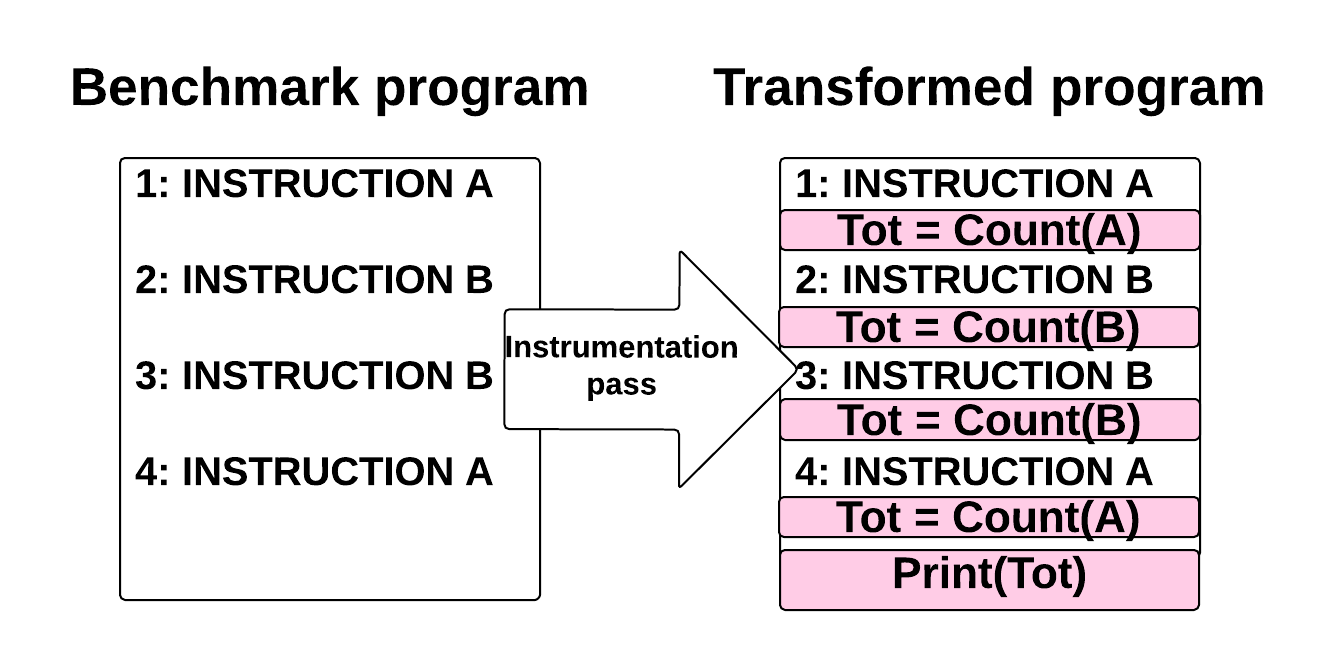
\includegraphics[width=0.4\textwidth]{CompilersProj1Part2Diag.png}
\caption{Required bytecode transformation}
\label{Part2transform}
\end{figure}

With a target binary defined we describe a code transformation that the opt pass must perform:
\begin{algorithm}
 \KwIn{$I$}
 $x \gets 0$\\
 $i \gets$ ref($I$.at(0)) \\
 \While{$i + 1 \neq \0$}
 { 
 	
 	$i' \gets$ \textbf{Count}(valAt($i$))\\ 
 	$i$.insertBefore($i'$)\\
 	$i$ += 1\\
 }
 $i \gets$ ref($I$.last())\\
 $i$.insertBefore(\textbf{print}())

 \caption{Dynamic instruction count instrumentation pass}
\end{algorithm}
where:\\
$I$ is an input program instruction list in LLVM byte code (.bc) format\\
$i$ is an individual instruction iterator $I$\\

The \textit{count()} function can be recycled from section the \textit{static count} pass. Similarly the \textit{Print()} function can be recycled.

\subsection{Instrumentation pass implementation summary}
Besides the skills used for the static pass, implementation of the dynamic pass presented challenges of inserting instrumentation functions to the test bench code and further augmenting that code to call inserted functions.\\
Ensuring instrumentation functions were in scope during the opt pass was documented in the one of the project breif "hints" sections. Counting sorted lists of instructions was a probem solved during the static instruction count problem. Therefore the major challenges were: 
\begin{itemize}
\item Finding a function signature in LLVM byte code
\item Inserting a call to a function signature above a byte code instruction
\item Passing parameters to an inserted function call
\end{itemize}

Finding a function signature \textbf{COSTAS IMPROVED THIS, I WILL SAY NO MORE}\\

Inserting a function call 

\section{Profiling branch bias}

\subsection{Conclusions}

The project was completed succesfully . Learning outcomes were a working understanding of LLVM optimiser passes. We are capable of transforming and instrumenting code. We have developed an efficient method to develop, test and debug the LLVM source tree with a debug api and symbol indexed code base via the eclipse CDT. Understanding how to instrument code has provided a powerful tool for analysis of any optimisation heuristics applied by other opt passes. Instrumentation will allow us to both formulate and test heuristics based on the performance of compiled code.\\
To conclude, this project has provided us with a solid foundation for the second upcoming project for CSE 231

{\footnotesize \bibliographystyle{acm}
\bibliography{sample.bib}}


\theendnotes

\end{document}







